\documentclass[a4paper,landscape,25pt]{foils}
\usepackage{graphicx}

\title{5次魔方陣全解出力プログラムの \\ 並列化と性能評価}
\author{4年次 \\ 杉崎 行優}

\begin{document}
\maketitle

\foilhead[-.5in]{5次魔方陣}
\begin{itemize}
\item 定義
\begin{itemize}
\item 5 $\times$ 5 のマス目
\item 1 $\sim$ 25 の数が1つずつ入る
\item 縦の5列 $\cdot$ 横の5列 $\cdot$ 斜めの2列の合計が全て等しい(式\ref{eqn:l})
\begin{boldequation} \label{eqn:l}
L=\frac{1}{5}\sum_{i=1}^{25}i=\frac{5\times(25+1)}{2}=65
\end{boldequation}
\end{itemize}
\item 全解は2億7530万5224通り存在
\end{itemize}

\foilhead{5次魔方陣の例}
\begin{figure}[htb]
\centering
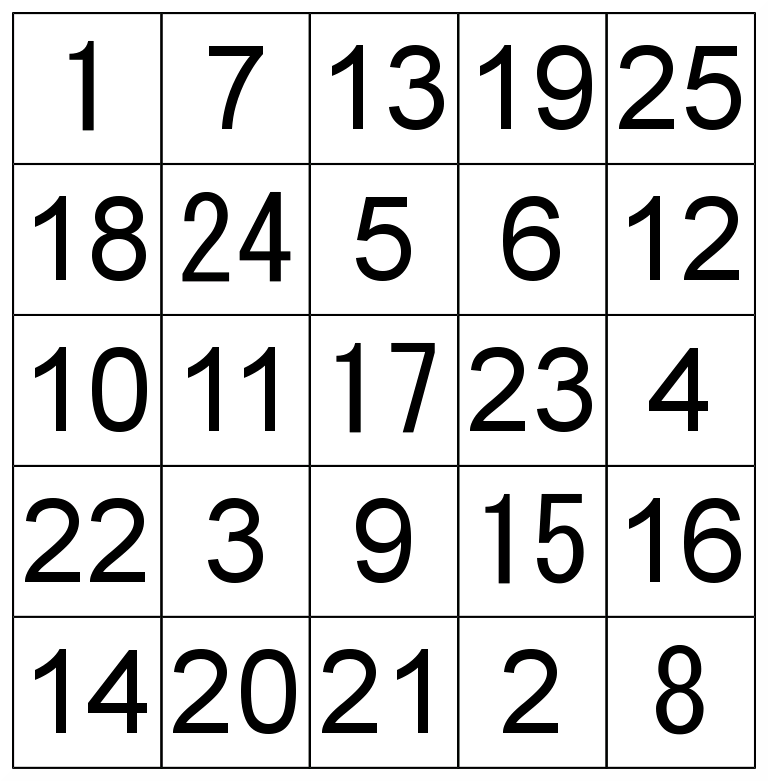
\includegraphics[height=0.7\textheight]{image1}
%%\caption{5次魔方陣の例}
\end{figure}

\foilhead{アルゴリズム}
\begin{itemize}
\item 全ての数字を総当たりで入れるのが基本
\item 列の和より、5マス中の4マスが埋まれば残りの1マスは自動的に求められる(枝刈り; バックトラッキング)
\begin{itemize}
\item 総当りするマスを14マスに減らす
\item 完全総当たりと比較し約$4\times10^7$倍高速化
\end{itemize}
\end{itemize}

\foilhead{並列化$(1)$}
\begin{itemize}
\item 並列方式 $\cdots$ マスタ$\cdot$ワーカー型並列
\begin{itemize}
\item 1コアをマスタ(司令塔)とする
\item その他のコアをワーカーとし、マスタの指示に従わせる
\end{itemize}
\end{itemize}

\foilhead{並列化$(2)$}
\begin{itemize}
\item マスタが$N$番目$(0 \ge N \ge 14)$のマスまで総当たりし、ワーカーがそれを受け取り、$N+1$番目のマスまで総当たり
\begin{itemize}
\item $N$の値が小さいとワーカーの粒度(仕事のバラつき)が大きくなり、ワーカーの計算時間がバラつく
\item $N$の値が大きいと粒度が小さくなりワーカーの計算時間が均等になるが、通信のコストが増大
\end{itemize}
\end{itemize}

\foilhead{実験環境}
\begin{itemize}
\item 筑波大学のスーパーコンピュータT2K-Tsukuba
\item 512CPUコア(32ノード)
\item 実行時間の制限より、$N$を3から8とした
\end{itemize}

\foilhead{実験結果}
\begin{itemize}
\newpage
\begin{figure}[htb]
\centering
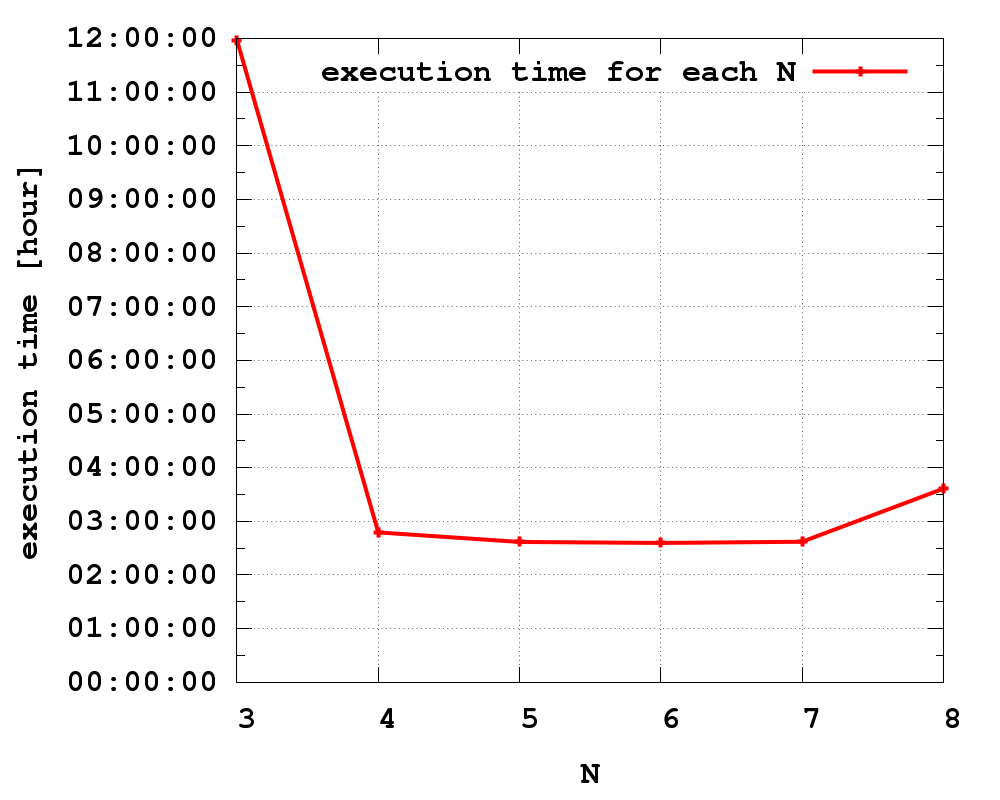
\includegraphics[height=0.7\textheight]{image3}
\caption{各$N$における全体実行時間}
\end{figure}
\item 実行時間は$N=3, \ 8$で長く、$N=6$で最短
\end{itemize}

\foilhead{考察(1)$\cdots$$N=3$}
\begin{figure}[htb]
\centering
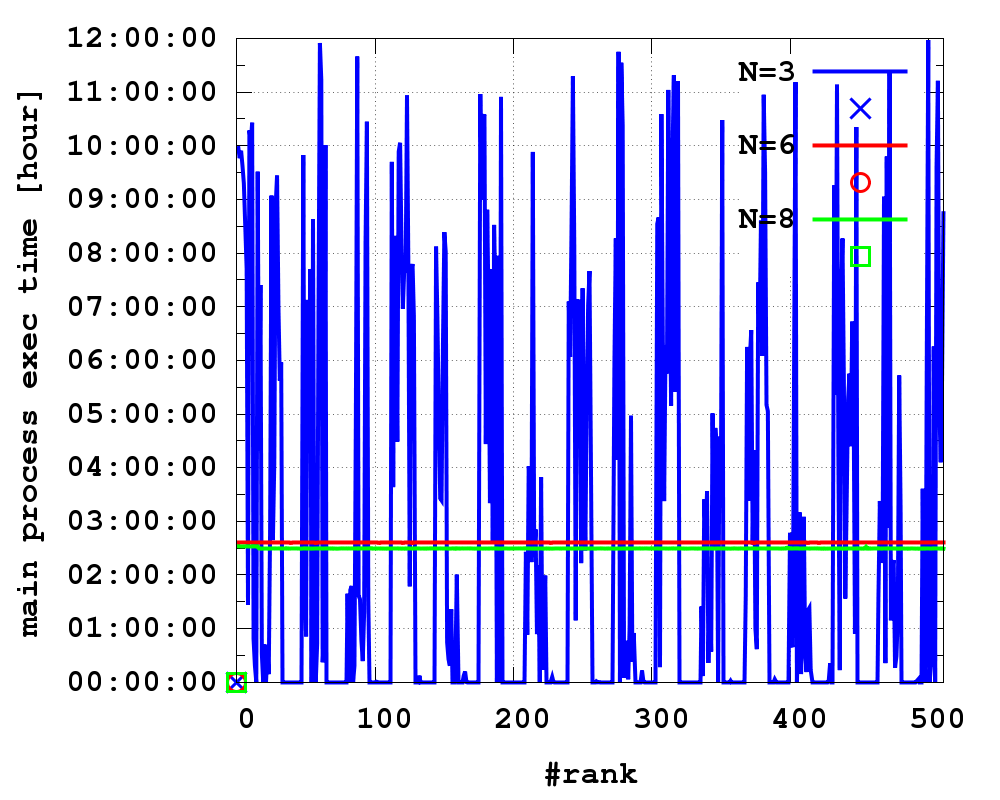
\includegraphics[height=0.7\textheight]{image4}
\caption{各ワーカーの主要処理実行時間}
\end{figure}
\begin{itemize}
\item 各ワーカーの主要処理時間に大きなバラつきが見られる
\end{itemize}

\foilhead{考察(2)$\cdots$$N=8$}
\begin{figure}[htb]
\centering
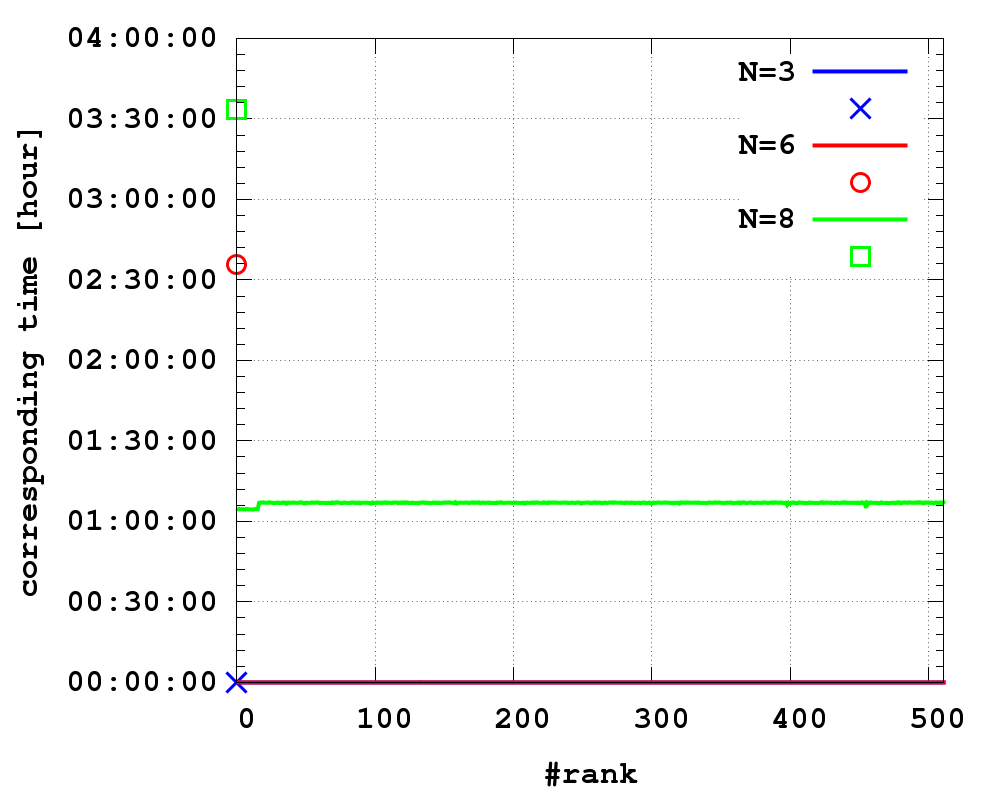
\includegraphics[height=0.7\textheight]{image5}
\caption{各ワーカーの総通信時間}
\end{figure}
\begin{itemize}
\item 総通信時間が約1時間と、長い
\end{itemize}

\foilhead{考察(3)$\cdots$$N=6$}
\begin{itemize}
\item 問題の粒度と通信のバランスがとれており、実行時間が最短になったと考えられる
\item 子曰「君子中庸。小人反中庸。...中庸其至矣乎。...」
\end{itemize}

\foilhead[-.5in]{今後の計画}
\begin{itemize}
\item 6次魔方陣への拡張
\begin{itemize}
\item 現在のプログラムを6次としてT2K-Tsukubaで実行した場合150兆年かかる
\item アルゴリズムやプログラムの大幅な改良がない限り、6次魔方陣の求解は不可能
\end{itemize}
\item (この先、魔方陣をテーマとし、かつ計算科学をやるというのは困難かもしれない$\cdots$)
\item (ここ数ヶ月の進捗がありません)
\end{itemize}

\foilhead{End of the sky}
Fragile


\end{document}
